\documentclass[11pt,a4paper]{article}
\usepackage{xcolor}
\usepackage{CJKutf8}
\usepackage{graphicx}
\usepackage{amsmath}
\usepackage{braket}
\usepackage{caption}
\usepackage{bm}
\usepackage{geometry}
\geometry{a4paper,scale=0.8}

\captionsetup{font={scriptsize}}

\begin{CJK}{UTF8}{gbsn}
\begin{document}

\title{Notes on quantum transport in mesoscopic systems}
\author{Li Gaoyang}
% \date{}
\date{\today}
\maketitle
\tableofcontents
% \newpage

\section{Basics}
\subsection{Magnon}
A magnon is a quasiparticle, a collective excitation of the electrons' spin structure in a crystal lattice. In the equivalent wave picture of quantum mechanics, a magnon can be viewed as a quantized spin wave. Magnons carry a fixed amount of energy and lattice momentum, and are spin-1, indicating they obey boson behavior.
\subsection{Hall effect}
\subsubsection{Conventional Hall effect}
\subsubsection{Quantum Hall effect}
\subsubsection{Spin Hall effect}
Occurs in paramagnetic systems as a result of spin-orbit interaction, refers to generation of pure spin current transverse to an applied electric field, even in the absence of magnetic field.

Similar to charge accumulation at sample edges in conventional Hall effect, spin accumulation is expected in spin Hall effect.
\begin{itemize}
\item extrinsic spin Hall effect: originates from asymmetric scattering for spin-up and spin-down.
\item intrinsic spin Hall effect: originates from band structures without scattering.\cite{ref1}
\end{itemize}
\subsubsection{Fractional Hall effect}
\subsubsection{Anomalous Hall effect}
\section{Formulas in PRB. 88, 220406(R) (2013)}
\subsection{Formula 1}
System Hamiltonion:
\begin{equation}
H=H_{L}+H_{R}+H_{s d}.
\end{equation}
Left lead is metallic
\begin{equation}
H_{L} = \sum_{k\sigma} \left(\varepsilon_{k\sigma}-\mu_{\sigma}\right) c_{k \sigma}^{\dagger} c_{k \sigma},
\end{equation}
right lead is insulating magnetic
\begin{equation}
H_{R} \approx \sum_{q} \hbar w_{q} a_{q}^{\dagger} a_{q}+\text { constant }.
\end{equation}
The interfacial electron-magnon interaction is described by
\begin{equation}
H_{s d}=-\sum_{k, q} J_{q}\left[S_{q}^{-} c_{k \uparrow}^{\dagger} c_{k+q \downarrow}+S_{q}^{+} c_{k+q \downarrow}^{\dagger} c_{k \uparrow}\right]
\end{equation}
where $S_{q}^{-} \approx \sqrt{2 S_{0}} a_{q}^{\dagger}, S_{q}^{+} \approx \sqrt{2 S_{0}} a_{q}$ are in the momentum space and $J_{q}$ denotes the effective exchange coupling at the interface. The magnonic spin current operator can be obtained by
\begin{equation}
\hat{I}_{S} = \frac{d\hat{N}_{R}}{dt} =  \frac{d}{dt} \sum_{q}a_{q}^{\dag}a_{q},
\end{equation}
the magnonic spin current is obtained by taking average over the nonequilibrium ground state $\ket{\psi_{0}}$ of the interacting system $H$:
\begin{equation}
I_{S} = \frac{dN_{R}}{dt} =  \frac{d}{dt} \langle \sum_{q}a_{q}^{\dag}a_{q}\rangle.
\end{equation}
Using the Heisenberg equation, we get
\begin{equation}
I_{S}=\frac{i}{\hbar}\langle[H_{s d}, \sum_{q} a_{q}^{\dagger} a_{q}]\rangle.
\end{equation}
\begin{equation}
[H_{s d}, \sum_{q} a_{q}^{\dagger} a_{q}] = [-\sum_{k, q} J_{q}\left(S_{q}^{-} c_{k \uparrow}^{\dagger} c_{k+q \downarrow}+S_{q}^{+} c_{k+q \downarrow}^{\dagger} c_{k \uparrow}\right), \sum_{q} a_{q}^{\dagger} a_{q}],
\end{equation}
in which,
\begin{equation}
[a_{q}^{\dag}, \sum_{q^{\prime}} a_{q'}^{\dagger}, a_{q^{\prime}}] = \delta_{q q^{\prime}}[a_{q}^{\dagger}, a_{q^{\prime}}^{\dagger} a_{q^{\prime}}] = [a_{q}^{\dagger}, a_{q}^{\dagger} a_{q}] = a_{q}^{\dagger}[a_{q}^{\dagger}, a_{q}] = - a_{q}^{\dagger}.
\end{equation}
Similarly,
\begin{equation}
[a_{q}, \sum_{q^{\prime}} a_{q^{\prime}}^{+} a_{q^{\prime}}]=[a_{q}, a_{q}^{\dagger} a_{q}]=a_{q}.
\label{eq:1-1}
\end{equation}
So,
\begin{equation}
\begin{split}
I_{S}&=\frac{i}{\hbar}\langle -\sum_{k q} J_{q}\left(-S_{q}^{-} c_{k \uparrow}^{\dagger} c_{k+q\downarrow} + S_{q}^{+} c_{k+q\downarrow}^{\dagger} c_{k \uparrow}\right) \rangle \\
&= \frac{i}{\hbar} \sum_{k q} J_{q}\left( \langle S_{q}^{-} c_{k \uparrow}^{\dagger} c_{k+q\downarrow}\rangle - \langle S_{q}^{+} c_{k+q\downarrow}^{\dagger} c_{k \uparrow}\rangle \right).
\end{split}
\end{equation}
\subsection{Formula 2}
\begin{equation}
\frac{d}{d t}\left\langle S_{q}^{+} c_{k+q \downarrow}^{\dagger} c_{k \uparrow}\right\rangle=\frac{i}{\hbar}\left\langle\left[H_{L}+H_{s d}+H_{R}, S_{q}^{+} c_{k+q \downarrow}^{\dagger} c_{k \uparrow}\right]\right\rangle.
\label{eq:2-1}
\end{equation}
The rhs. of eq. (\ref{eq:2-1}) is decomposed into 3 terms. The first term reads
\begin{equation}
\begin{split}
\left\langle\left[H_{L}, S_{q}^{+} c_{k+q \downarrow}^{\dagger} c_{k \uparrow}\right]\right\rangle &= [\sum_{k'\sigma}\left(\varepsilon_{k^{\prime}\sigma}-\mu_{\sigma}\right) c_{k' \sigma}^{\dagger} c_{k' \sigma}, S_{q}^{+} c_{k+q \downarrow}^{\dagger} c_{k \uparrow}] \\
&= S_{q}^{+} [\sum_{k'\sigma}\left(\varepsilon_{k^{\prime}\sigma}-\mu_{\sigma}\right) c_{k' \sigma}^{\dagger} c_{k' \sigma}, c_{k+q \downarrow}^{\dagger}]c_{k \uparrow} \\
&\quad + S_{q}^{+}c_{k+q \downarrow}^{\dagger}[\sum_{k'\sigma}\left(\varepsilon_{k^{\prime}\sigma}-\mu_{\sigma}\right) c_{k' \sigma}^{\dagger} c_{k' \sigma}, c_{k \uparrow}]
\end{split}
\end{equation}
Note that,
\begin{equation}
[\sum_{k^{\prime} \sigma} c_{k^{\prime} \sigma}^{\dag} c_{k^{\prime} \sigma}, c_{k+q \downarrow}^{\dagger}] = \sum_{k'\sigma} c_{k'\sigma}^{\dag}\delta_{k',k+q}\delta_{\sigma\downarrow} = c_{k+q\downarrow}^{\dag},
\label{eq:2-2}
\end{equation}
\begin{equation}
[\sum_{k^{\prime} \sigma} c_{k^{\prime} \sigma}^{\dag} c_{k^{\prime} \sigma}, c_{k \uparrow}] = - \sum_{k^{\prime} \sigma} \{c_{k'\sigma}^{\dag}, c_{k\uparrow}\}c_{k'\sigma} = - c_{k\uparrow}.
\label{eq:2-3}
\end{equation}
Eq. (\ref{eq:2-2}) (\ref{eq:2-3}) are derived using equity
\begin{equation}
\begin{split}
[AB, C] &= A[B, C] + [A, C]B \\
&= A\{B, C\} - \{A, C\}B.
\end{split}
\end{equation}
So,
\begin{equation}
\begin{split}
\left[H_{L}, S_{q}^{+} c_{k+q \downarrow}^{\dagger} c_{k \uparrow}\right] &= \left(\varepsilon_{k+q \downarrow}-\varepsilon_{k \uparrow}+\mu_{\uparrow}-\mu_{\downarrow}\right)S_{q}^{+} c_{k+q \downarrow}^{\dagger} c_{k \uparrow}.
\end{split}
\label{eq:1-0}
\end{equation}
If $\mu_{\uparrow} = \mu_{\downarrow}$, then eq. (\ref{eq:1-0}) reduces to
\begin{equation}
\begin{split}
\left[H_{L}, S_{q}^{+} c_{k+q \downarrow}^{\dagger} c_{k \uparrow}\right] &= \left(\varepsilon_{k+q \downarrow}-\varepsilon_{k \uparrow}\right)S_{q}^{+} c_{k+q \downarrow}^{\dagger} c_{k \uparrow}.
\end{split}
\label{eq:1-01}
\end{equation}
The second term $H_{R} = \sum_{q} \hbar w_{q} a_{q}^{\dagger} a_{q}$, then using eq. (\ref{eq:1-1}), we get
\begin{equation}
\left[H_{R}, S_{q}^{+} c_{k+q \downarrow}^{\dagger} c_{k \uparrow}\right] = -\hbar \omega_{q}S_{q}^{+} c_{k+q \downarrow}^{\dagger} c_{k \uparrow}.
\end{equation}
The third term in eq. (\ref{eq:2-1}) reads
\begin{equation}
\begin{split}
\left[H_{sd}, S_{q}^{+} c_{k+q \downarrow}^{\dagger} c_{k \uparrow}\right] &= - J_{q} \left[S_{q}^{-} c_{k \uparrow}^{\dagger} c_{k+q \downarrow}, S_{q}^{+} c_{k+q \downarrow}^{\dagger} c_{k \uparrow}\right] \\
&= J_{q} \left[S_{q}^{+} c_{k+q \downarrow}^{\dagger} c_{k \uparrow}, S_{q}^{-} c_{k \uparrow}^{\dagger} c_{k+q \downarrow}\right]
\end{split}
\end{equation}
Combine these three terms, we get
\begin{equation}
\begin{split}
\frac{d}{d t}\left\langle S_{q}^{+} c_{k+q \downarrow}^{\dagger} c_{k \uparrow}\right\rangle&=\frac{i}{\hbar}\left(\varepsilon_{k+q \downarrow}-\varepsilon_{k \uparrow}-\hbar \omega_{q}\right)\left\langle S_{q}^{+} c_{k+q \downarrow}^{\dagger} c_{k \uparrow}\right\rangle\\ 
&\quad + \frac{i}{\hbar} J_{q}\left\langle\left[S_{q}^{+} c_{k+q \downarrow}^{\dagger} c_{k \uparrow}, S_{q}^{-} c_{k \uparrow}^{\dagger} c_{k+q \downarrow}\right]\right\rangle,
\end{split}
\end{equation}
which is also eq. (2) in PRB. 88, 220406(R) (2013).

\section{Spin current in NM-QD-MIL system}
For system consists of quantum dot(QD) sandwiched by a left normal metal(NM) lead and a right magnetic insulating lead(MIL), the Hamiltonian is
\begin{equation}
H=H_{\rm{L}}+H_{\rm{QD}}+H_{\rm{R}}+H_{\rm{T}}.
\end{equation}

\begin{equation}
H_{\rm{L}} = \sum_{k\sigma} \varepsilon_{k\sigma} c_{k \sigma}^{\dagger} c_{k \sigma},
\end{equation}

\begin{equation}
H_{\rm{QD}} = \sum_{\sigma}\varepsilon_{\sigma} d_{\sigma}^{\dagger} d_{\sigma},
\end{equation}

\begin{equation}
H_{\rm{R}} \approx \sum_{q} \hbar w_{q} a_{q}^{\dagger} a_{q},
\end{equation}

\begin{equation}
H_{\rm{T}} = V_{\rm{L}} + V_{\rm{R}}
\end{equation}
V$_{L}$ is the coupling between left lead and QD, while V$_{R}$ is the coupling between right lead and QD.
\begin{equation}
V_{\rm{L}} = \sum_{k\sigma}( t_{k\sigma} c_{k \sigma}^{\dagger} d_{\sigma} + t_{k\sigma}^{*} d_{\sigma}^{\dagger} c_{k\sigma})
\end{equation}

\begin{equation}
V_{\rm{R}}=-\sum_{q} J_{q}\left[S_{q}^{-} d_{\uparrow}^{\dagger} d_{\downarrow}+S_{q}^{+} d_{\downarrow}^{\dagger} d_{\uparrow}\right].
\end{equation}

where $S_{q}^{-} \approx \sqrt{2 S_{0}} a_{q}^{\dagger}, S_{q}^{+} \approx \sqrt{2 S_{0}} a_{q}$ are in the momentum space and $J_{q}$ denotes the effective exchange coupling between the QD and MIL.
\subsection{Spin-dependent current in left lead}
The spin-dependent current flow out of left lead is $I_{L\sigma}$:
\begin{equation}
I_{L\sigma} = \frac{d}{dt} \langle N_{L\sigma} \rangle
\end{equation}
in which, $N_{L\sigma} = \sum_{k} c_{k\sigma}^{\dag}c_{k\sigma}$
Heisenberg equation:
\begin{equation}
\frac{d}{dt} \langle N_{L\sigma} \rangle = \frac{i}{\hbar} \langle [H, N_{L\sigma}]\rangle
\end{equation}

\begin{equation}
[H, N_{L\sigma}] = [H_{T}, N_{L\sigma}] =  \sum_{k}\left(t_{k \sigma}^{*} d_{\sigma}^{\dagger} c_{k \sigma} - t_{k \sigma} c_{k \sigma}^{\dagger} d_{\sigma} \right)
\end{equation}
so, the spin-dependent current
\begin{equation}
I_{L\sigma} = \frac{i}{\hbar} \sum_{k} \left( t_{k \sigma}^{*} \langle  d_{\sigma}^{\dagger} c_{k \sigma}\rangle - t_{k \sigma} \langle c_{k \sigma}^{\dagger} d_{\sigma} \rangle \right).
\end{equation}
Namely, the spin-up current is
\begin{equation}
I_{L\uparrow} = \frac{i}{\hbar} \sum_{k} \left( t_{k \uparrow}^{*} \langle  d_{\uparrow}^{\dagger} c_{k \uparrow}\rangle - t_{k \uparrow} \langle c_{k \uparrow}^{\dagger} d_{\uparrow} \rangle \right),
\end{equation}
the spin-down current is
\begin{equation}
I_{L\downarrow} = \frac{i}{\hbar} \sum_{k} \left( t_{k \downarrow}^{*} \langle  d_{\downarrow}^{\dagger} c_{k \downarrow}\rangle - t_{k \downarrow} \langle c_{k \downarrow}^{\dagger} d_{\downarrow} \rangle \right),
\end{equation}
The charge current in left lead is defined as
\begin{equation}
I_{e} = e(I_{L\uparrow} + I_{L\downarrow}).
\end{equation}
The spin current in left lead is defined as
\begin{equation}
I_{LS} = \frac{1}{2}(I_{L\uparrow} - I_{L\downarrow})
\end{equation}
Substitute the spin-dependent current in, we get the spin current in left lead
\begin{equation}
I_{LS} = \frac{i}{2\hbar} \sum_{k} \left( t_{k \uparrow}^{*} \langle  d_{\uparrow}^{\dagger} c_{k \uparrow}\rangle - t_{k \uparrow} \langle c_{k \uparrow}^{\dagger} d_{\uparrow} \rangle -  t_{k \downarrow}^{*} \langle  d_{\downarrow}^{\dagger} c_{k \downarrow}\rangle + t_{k \downarrow} \langle c_{k \downarrow}^{\dagger} d_{\downarrow} \rangle \right)
\end{equation}
\subsection{magnonic current in right lead}
The magnonic current in right lead is
\begin{equation}
I_{RS} = \frac{d\langle N_{R}\rangle}{dt} =  \frac{d}{dt} \langle \sum_{q}a_{q}^{\dag}a_{q}\rangle,
\end{equation}
From the Heisenberg equation, we have
\begin{equation}
\frac{d}{dt} \langle \sum_{q}a_{q}^{\dag}a_{q}\rangle = \frac{i}{\hbar} \langle [H, \sum_{q}a_{q}^{\dag}a_{q}] \rangle.
\end{equation}
We have
\begin{equation}
\begin{split}
&[H, \sum_{q}a_{q}^{\dag}a_{q}] \\
= &[V_{R}, \sum_{q}a_{q}^{\dag}a_{q}]\\
= &-\sum_{q} J_{q} \Big(\big[S_{q}^{-}d_{\uparrow}^{\dag}d_{\downarrow}, \sum_{q'}a_{q'}^{\dag}a_{q'}\big] + \big[S_{q}^{+}d_{\downarrow}^{\dag}d_{\uparrow}, \sum_{q'}a_{q'}^{\dag}a_{q'}\big]\Big) \\
= & \sum_{q} J_{q} \big( S_{q}^{-}d_{\uparrow}^{\dag}d_{\downarrow} - S_{q}^{+}d_{\downarrow}^{\dag}d_{\uparrow} \big)
\end{split}
\end{equation}
So, the magnon current reads
\begin{equation}
I_{RS} = \frac{i}{\hbar} \sum_{q} J_{q} \big( \big\langle S_{q}^{-}d_{\uparrow}^{\dag}d_{\downarrow}\big\rangle - \big\langle S_{q}^{+}d_{\downarrow}^{\dag}d_{\uparrow} \big\rangle \big) .
\end{equation}

\subsection{spin-dependent current in QD}
Similarly, the spin-dependent current in the central QD is defined as
\begin{equation}
I_{C\sigma} = \langle\frac{dN_{C\sigma}}{dt} \rangle= \langle  \frac{d}{dt} d_{\sigma}^{\dag}d_{\sigma}\rangle,
\end{equation}
Heisenberg equation:
\begin{equation}
\frac{d}{dt} d_{\sigma}^{\dag}d_{\sigma} = \frac{i}{\hbar} [H, d_{\sigma}^{\dag}d_{\sigma}].
\end{equation}
Specifically, we have
\begin{equation}
 [H, d_{\sigma}^{\dag}d_{\sigma}] = [V_{L},  d_{\sigma}^{\dag}d_{\sigma}] + [V_{R},  d_{\sigma}^{\dag}d_{\sigma}]
\end{equation}
in which,
\begin{equation}
\begin{split}
[V_{L},  d_{\sigma}^{\dag}d_{\sigma}] &= \sum_{k'\sigma'}\big(t_{k'\sigma'} \big[c_{k'\sigma'}^{\dag}d_{\sigma'},  d_{\sigma}^{\dag}d_{\sigma}\big] + t_{k'\sigma'}^{*} \big[d_{\sigma'}^{\dag}c_{k'\sigma'},  d_{\sigma}^{\dag}d_{\sigma}\big] \big) \\
&  = \sum_{k'\sigma'}\big(t_{k'\sigma'} c_{k'\sigma'}^{\dag}d_{\sigma'}\delta_{\sigma\sigma'} - t_{k'\sigma'}^{*} d_{\sigma'}^{\dag}c_{k'\sigma'} \delta_{\sigma\sigma'}\big) \\
&= \sum_{k}\big(t_{k\sigma} c_{k\sigma}^{\dag}d_{\sigma} - t_{k\sigma}^{*} d_{\sigma}^{\dag}c_{k\sigma} \big)
\end{split}
\end{equation}
We change the summation index from $k'$ to $k$ in the last line , which doesn't change the result.
\begin{equation}
[V_{R},  d_{\sigma}^{\dag}d_{\sigma}] = -\sum_{q}J_{q}\big( S_{q}^{-} \big[d_{\uparrow}^{\dag}d_{\downarrow}, d_{\sigma}^{\dag}d_{\sigma} \big] + S_{q}^{+}\big[d_{\downarrow}^{\dag}d_{\uparrow}, d_{\sigma}^{\dag}d_{\sigma} \big]\big)
\end{equation}
in which,
\begin{equation}
\begin{split}
\big[d_{\uparrow}^{\dag}d_{\downarrow}, d_{\sigma}^{\dag}d_{\sigma} \big] &= d_{\uparrow}^{\dag} \big[d_{\downarrow}, d_{\sigma}^{\dag}d_{\sigma}\big] + \big[d_{\uparrow}^{\dag} , d_{\sigma}^{\dag}d_{\sigma} \big]d_{\downarrow} \\
&=d_{\uparrow}^{\dag}d_{\downarrow}\delta_{\sigma \downarrow} - d_{\uparrow}^{\dag}d_{\downarrow}\delta_{\sigma \uparrow}
\end{split}
\end{equation}
So,
\begin{equation}
[V_{R},  d_{\sigma}^{\dag}d_{\sigma}] =  -\sum_{q}J_{q}\big[ S_{q}^{-} \big( d_{\uparrow}^{\dag}d_{\downarrow}\delta_{\sigma \downarrow} - d_{\uparrow}^{\dag}d_{\downarrow}\delta_{\sigma \uparrow} \big) + S_{q}^{+}\big(d_{\downarrow}^{\dag}d_{\uparrow}\delta_{\sigma \uparrow} - d_{\downarrow}^{\dag}d_{\uparrow}\delta_{\sigma \downarrow} \big)\big]
\end{equation}
The spin-dependent current is
\begin{eqnarray}
I_{C\uparrow} = \frac{i}{\hbar}\big[ H, d_{\uparrow}^{\dag} d_{\uparrow} \big]
\\
I_{C\downarrow} = \frac{i}{\hbar}\big[ H, d_{\downarrow}^{\dag} d_{\downarrow} \big]
\end{eqnarray}
which gives
\begin{equation}
I_{C\uparrow} = \frac{i}{\hbar} \big[ \sum_{k}\big(t_{k\uparrow} c_{k\uparrow}^{\dag}d_{\uparrow} - t_{k\uparrow}^{*} d_{\uparrow}^{\dag}c_{k\uparrow} \big) + \sum_{q}J_{q}\big( S_{q}^{-} d_{\uparrow}^{\dag}d_{\downarrow} - S_{q}^{+}d_{\downarrow}^{\dag}d_{\uparrow} \big)\big]
\end{equation}
and
\begin{equation}
I_{C\downarrow} = \frac{i}{\hbar} \big[ \sum_{k}\big(t_{k\downarrow} c_{k\downarrow}^{\dag}d_{\downarrow} - t_{k\downarrow}^{*} d_{\downarrow}^{\dag}c_{k\downarrow} \big) + \sum_{q}J_{q}\big(S_{q}^{+}d_{\downarrow}^{\dag}d_{\uparrow} -  S_{q}^{-} d_{\uparrow}^{\dag}d_{\downarrow} \big)\big].
\end{equation}
The spin current in central dot is
\begin{equation}
I_{CS} = \frac{1}{2}(I_{C\uparrow} - I_{C\downarrow})
\end{equation}

\subsection{Verifying continuity condition}
\subsubsection{Charge current}
Since the right lead is a insulating lead, there is no charge current flow through it, so the charge current is
\begin{equation}
I_{Re} = 0
\end{equation}
where the subscript R denotes the right lead, while the subscript e denotes the charge current.

Meanwhile, the charge current flows in left lead and QD is
\begin{equation}
I_{e} = e(\sum_{\sigma}I_{L\sigma} + \sum_{\sigma}I_{C\sigma}) = 0
\end{equation}
\subsubsection{Spin current}
Spin current in the left lead and QD:
\begin{equation}
I_{LS} + I_{CS} = \frac{i}{\hbar} \sum_{q} J_{q} \big( \big\langle S_{q}^{-}d_{\uparrow}^{\dag}d_{\downarrow}\big\rangle - \big\langle S_{q}^{+}d_{\downarrow}^{\dag}d_{\uparrow} \big\rangle \big) .
\end{equation}
The magnon current is
\begin{equation}
I_{RS} = \frac{i}{\hbar} \sum_{q} J_{q} \big( \big\langle S_{q}^{-}d_{\uparrow}^{\dag}d_{\downarrow}\big\rangle - \big\langle S_{q}^{+}d_{\downarrow}^{\dag}d_{\uparrow} \big\rangle \big) ,
\end{equation}
in which, $I_{LS}, I_{CS}, I_{RS}$ is defined earlier. Thus, we have
\begin{equation}
\begin{split}
I_{LS} + I_{CS} &= I_{RS}\\
& = \frac{i}{\hbar} \sum_{q} J_{q} \big( \big\langle S_{q}^{-}d_{\uparrow}^{\dag}d_{\downarrow}\big\rangle - \big\langle S_{q}^{+}d_{\downarrow}^{\dag}d_{\uparrow} \big\rangle \big) .
\end{split}
\end{equation}
\subsection{Perturbation expansion of $G_{d}(\tau, \tau)$}
When neglecting left lead, the hamiltonian is
\begin{equation}
H = H_{QD} + H_{R} + H_{sd}
\end{equation}
Expand S-matrix up to the second order of J, we have
\begin{equation}
\begin{split}
&G_{d}(\tau, \tau) = -i\langle T_{C}Ss_{q}^{+}(\tau)s_{q}^{-}(\tau') \rangle \\
=& -i\sum_{k} g_{k\uparrow}(\tau', \tau) g_{k+q\downarrow}(\tau, \tau') \\
+& \int_{c}d\tau_{1}\int_{c}d\tau_{2} \sum_{kq_{1}} J_{q_{1}}^{2} g_{Rq_{1}}(\tau_{2}, \tau_{1}) g_{k\uparrow}(\tau', \tau_{2}) g_{k+q_{1}\downarrow}(\tau_{2}, \tau_{1}) g_{k\uparrow}(\tau_{1}, \tau) g_{k+q\downarrow}(\tau, \tau') \\
+& \int_{c}d\tau_{1}\int_{c}d\tau_{2} \sum_{kq_{1}} J_{q_{1}}^{2} g_{Rq_{1}}(\tau_{2}, \tau_{1}) g_{k\uparrow}(\tau', \tau) g_{k+q\downarrow}(\tau, \tau_{1}) g_{k+q-q_{1}\uparrow}(\tau_{1}, \tau_{2}) g_{k+q\downarrow}(\tau_{2}, \tau') \\
-& \int_{c}d\tau_{1}\int_{c}d\tau_{2} \sum_{kk'} J_{q}^{2} g_{Rq}(\tau_{2}, \tau_{1}) g_{k\uparrow}(\tau_{1}, \tau) g_{k+q\downarrow}(\tau, \tau_{1})  g_{k'\uparrow}(\tau', \tau_{2}) g_{k'+q\downarrow}(\tau_{2}, \tau')
\end{split}
\end{equation}
\section{Checking formulas in notes}
% \documentclass[11pt,a4paper]{article}
\usepackage{xcolor}
\usepackage{CJKutf8}
\usepackage{graphicx}
\usepackage{amsmath}
\usepackage{braket}
\usepackage{caption}
\usepackage{bm}
\usepackage{geometry}
\geometry{a4paper,scale=0.8}

\captionsetup{font={scriptsize}}

\begin{CJK}{UTF8}{gbsn}
\begin{document}

\title{NEGF Notes}
% \author{Li Gaoyang}
% \date{}
\date{\today}
\maketitle
% \tableofcontents

% \newpage

\subsection{Hamiltonian}
\begin{equation}
H=H_{L}+H_{R}+H_{d}+H_{T}+H_{s d}
\end{equation}
\begin{equation}
H_{L}=\sum_{k \sigma} \epsilon_{k \sigma, L} c_{k \sigma}^{\dagger} c_{k \sigma}
\end{equation}
\begin{equation}
H_{R}=\sum_{q} \omega_{q} a_{q}^{\dagger} a_{q}
\end{equation}
\begin{equation}
H_{d}=\sum_{n \sigma} \epsilon_{n \sigma} d_{n \sigma}^{\dagger} d_{n \sigma}
\end{equation}
\begin{equation}
H_{T}=\sum_{k \sigma n}\left(t_{k \sigma n} c_{k \sigma}^{\dagger} d_{n \sigma}+t_{k \sigma n}^{*} d_{n \sigma}^{\dagger} c_{k \sigma}\right)
\end{equation}
\begin{equation}
H_{s d}=-\sum_{q n m} J_{q}\left(d_{n \uparrow}^{\dagger} d_{m \downarrow} a_{q}^{\dagger}+a_{q} d_{m \downarrow}^{\dagger} d_{n \uparrow}\right) \delta\left(\epsilon_{n \uparrow}-\epsilon_{m \downarrow}-\omega_{q}\right)
\end{equation}
\begin{equation}
s_{q}^{+}=\sum_{n m} d_{n \uparrow}^{\dagger} d_{m \downarrow} \delta_{\uparrow \downarrow}
\end{equation}
\begin{equation}
s_{q}^{-}=\sum_{n m} d_{m \downarrow}^{\dagger} d_{n \uparrow} \delta_{\uparrow \downarrow}
\end{equation}
\subsubsection{check operators}
\begin{equation}
i \dot{a}_{q}=\omega_{q} a_{q}-J_{q} s_{q}^{+}
\end{equation}
\begin{equation}
i \dot{c}_{k \sigma}=\epsilon_{k \sigma, L} c_{k \sigma}+\sum_{k^{\prime}} t_{k \sigma n} d_{n \sigma}
\end{equation}
\begin{equation}
i \dot{d}_{n \uparrow}=\epsilon_{n \uparrow} d_{n \uparrow}+\sum_{k} t_{k \uparrow n}^{*} c_{k \uparrow}-\sum_{q, m} J_{q} a_{q}^{\dagger}d_{m \downarrow}\delta(\epsilon_{n \uparrow}-\epsilon_{m \downarrow}-\omega_{q})
\end{equation}
\begin{equation}
i \dot{d}_{n \downarrow}=\epsilon_{n \downarrow} d_{n \downarrow}+\sum_{k} t_{k \downarrow n}^{*} c_{k \downarrow}-\sum_{q, m} J_{q} a_{q}d_{m \uparrow}\delta(\epsilon_{m \uparrow}-\epsilon_{n \downarrow}-\omega_{q})
\end{equation}
\subsection{spin current ???}
Define
\begin{equation}
G_{d, R}\left(\tau, \tau^{\prime}\right)=-i\langle s_{q}^{+}(\tau) a_{q}^{\dag}(\tau')\rangle.
\end{equation}
The lesser Green's function is($s_{q}^{+}$ is fermionic but $a_{q}$ is bosonic)
\begin{equation}
G_{d, R}^{<}\left(t, t'\right)=-i\langle  a_{q}^{\dag}(t') s_{q}^{+}(t) \rangle
\end{equation}
We also define the Green’s function that is related to the QD (not the Green’s function of the QD),
\begin{equation}
G_{d}\left(\tau, \tau^{\prime}\right)= -i\left\langle T_{c} S s_{q}^{+}(\tau) s_{q}^{-}\left(\tau^{\prime}\right)\right\rangle .
\end{equation}
We have
\begin{equation}
-i \partial_{\tau^{\prime}} G_{d, R}\left(\tau, \tau^{\prime}\right)=\omega_{q} G_{d, R}\left(\tau, \tau^{\prime}\right)-J_{q} G_{d}
\end{equation}
or
\begin{equation}
G_{d, R} g_{R q}^{-1}=-J_{q} G_{d}
\end{equation}
or
\begin{equation}
G_{d, R}\left(\tau, \tau^{\prime}\right)=-J_{q} \int G_{d}\left(\tau, \tau_{1}\right) g_{R q}\left(\tau_{1}, \tau^{\prime}\right) d \tau_{1}
\end{equation}
the minus before $J_{q}$ originates from the minus in $H_{sd}$. The rules of analytic continuation gives
\begin{equation}
G_{d, R}^{<}\left(t, t^{\prime}\right)=-J_{q} \int_{-\infty}^{\infty}dt_{1} [G_{d}^{r}\left(t, t_{1}\right) g_{R q}^{<}\left(t_{1}, t^{\prime}\right) + G_{d}^{<}\left(t, t_{1}\right) g_{R q}^{a}\left(t_{1}, t^{\prime}\right)]
\end{equation}
and
\begin{equation}
G_{R,d}^{<}\left(t, t^{\prime}\right)=-J_{q} \int_{-\infty}^{\infty}dt_{1} [g_{R q}^{r}\left(t, t_{1}\right) G_{d}^{<}\left(t_{1}, t'\right)  + g_{R q}^{<}\left(t, t_{1}\right) G_{d}^{a}\left(t_{1}, t'\right)]
\end{equation}
The spin current flows out of right lead is
\begin{equation}
\begin{split}
I_{s}&= i \sum_{q} J_{q}\left(\left\langle s_{q}^{+} a_{q}^{\dagger}\right\rangle-\left\langle a_{q} s_{q}^{-}\right\rangle\right) \\
&=-\sum_{q}J_{q}(G_{d,R}^{<}(t,t)-G_{R,d}^{<}(t,t)) \\
&=2\rm{Re}\sum_{q} \int  d t_{1}\operatorname{Tr}\left[G_{d}^{r}\left(t, t_{1}\right) \Sigma_{Rq}^{<}\left(t_{1}, t^{\prime}\right)+G_{d}^{<}\left(t, t_{1}\right) \Sigma_{Rq}^{a}\left(t_{1}, t^{\prime}\right)\right]
% \\ &=2\rm{Re}\sum_{q} \int  d t_{1}\operatorname{Tr}\left[\left(G_{d}^{>}-G_{d}^{<}\right) \Sigma_{R q}^{<}+G_{d}^{<}\left(\Sigma_{R q}^{a}-\Sigma_{R q}^{r}\right)\right]
\end{split}
\end{equation}
\begin{equation}
\Sigma_{Rq}^{\gamma}(\tau, \tau')=J_{q}^{2}g_{Rq}^{\gamma}(\tau, \tau')
\end{equation}
\subsection{Calculation of $G_{d}$}
Definition:
\begin{equation}
\begin{split}
G_{d}\left(\tau, \tau^{\prime}\right)&=
-i\left\langle T_{c} S s_{q}^{+}(\tau) s_{q}^{-}\left(\tau^{\prime}\right)\right\rangle \\
&=-i\sum_{mnm'n'}\langle T_{c}S d_{n \uparrow}^{\dagger} d_{m \downarrow} d_{m' \downarrow}^{\dagger} d_{n' \uparrow} \rangle \delta\left(\epsilon_{n \uparrow}-\epsilon_{m \downarrow}-\omega_{q}\right) \delta\left(\epsilon_{n' \uparrow}-\epsilon_{m' \downarrow}-\omega_{q}\right) 
\end{split}
\end{equation}
When right lead is absent, the system Hamiltonian is
\begin{equation}
H = H_{L} + H_{d} + H_{T}.
\end{equation}
\begin{equation}
G_{d}\left(\tau, \tau^{\prime}\right)=-i\sum_{mnm'n'}G_{L,n'n\uparrow}(\tau', \tau) G_{L,mm'\downarrow}(\tau, \tau') \delta\left(\epsilon_{n \uparrow}-\epsilon_{m \downarrow}-\omega_{q}\right) \delta\left(\epsilon_{n' \uparrow}-\epsilon_{m' \downarrow}-\omega_{q}\right)
\end{equation}
where
\begin{equation}
\begin{split}
G_{L,mn\sigma}(\tau, \tau')&= -i\langle T_{c}d_{m\sigma}(\tau) d_{n\sigma}^{\dag}(\tau')\rangle \\
&=g_{mn\sigma}(\tau, \tau')\delta_{mn} \\
&~~~+ \iint d\tau_{1}d\tau_{2} g_{mm\sigma}(\tau, \tau_{2}) \sum_{k} t_{k\sigma n}t_{k\sigma m}^{*} g_{k\sigma}(\tau_{2}, \tau_{1}) g_{nn\sigma}(\tau_{1}, \tau') \\
&~~~ +\cdots \\
&=g_{mn\sigma}(\tau, \tau')\delta_{mn} + \iint d\tau_{1}d\tau_{2} g_{mm\sigma}(\tau, \tau_{2}) \Sigma_{L,mn\sigma}(\tau_{2}, \tau_{1}) g_{nn\sigma}(\tau_{1}, \tau')\\
&~~~+ \cdots \\
&= 1 /\left[g_{mn \sigma}^{-1}-\Sigma_{L,mn \sigma}\right]
\end{split}
\end{equation}
\begin{equation}
g_{mn\sigma}(\tau, \tau') = -i\langle T_{c}d_{m\sigma}(\tau) d_{n\sigma}^{\dag}(\tau')\rangle_{0}
\end{equation}
Self-energy of left lead
\begin{equation}
\Sigma_{L,mn\sigma}(\tau_{2}, \tau_{1}) = \sum_{k} t_{k\sigma n}t_{k\sigma m}^{*} g_{k\sigma}(\tau_{2}, \tau_{1})
\end{equation}
where
\begin{equation}
g_{k\sigma}(\tau_{2}, \tau_{1}) = -i\langle T_{c}c_{k\sigma}(\tau_{2}) c_{k\sigma}^{\dag}(\tau_{1})\rangle_{0}.
\label{eq:left-self-energy}
\end{equation}
When left lead is absent, system Hamiltonian is
\begin{equation}
H = H_{d} + H_{R} + H_{sd}.
\end{equation}
\begin{equation}
\begin{split}
G_{d}\left(\tau, \tau^{\prime}\right) =&-i\sum_{mn} g_{n \uparrow}\left(\tau^{\prime}, \tau\right) g_{m \downarrow}\left(\tau, \tau^{\prime}\right) \delta(\varepsilon_{n\uparrow} - \varepsilon_{m\downarrow} - \omega_{q})\\
&-\int d\tau_{1}\int d\tau_{2} \sum_{mnm'n'}g_{n \uparrow}\left(\tau_{1}, \tau\right) g_{m \downarrow}\left(\tau, \tau_{1}\right) \Sigma_{R,mnm'n' }\left(\tau_{1}, \tau_{2}\right) g_{n'\uparrow}\left(\tau^{\prime}, \tau_{2}\right)g_{m'\downarrow}(\tau_{2}, \tau') \\
&~~~\times \delta(\varepsilon_{n\uparrow} - \varepsilon_{m\downarrow} - \omega_{q_{1}})\delta(\varepsilon_{n'\uparrow} - \varepsilon_{m'\downarrow} - \omega_{q_{1}})\\
& + \cdots \\
=& g_{d}(\tau, \tau') + \iint d\tau_{1}d\tau_{2}g_{d}(\tau, \tau_{1}) \Sigma_{R}(\tau_{1}, \tau_{2}) G_{d}(\tau_{2}, \tau')
\end{split}
\end{equation}
in which, 
\begin{equation}
g_{d}\left(\tau, \tau^{\prime}\right) = -i\sum_{mn} g_{n \uparrow}\left(\tau^{\prime}, \tau\right) g_{m \downarrow}\left(\tau, \tau^{\prime}\right) \delta(\varepsilon_{n\uparrow} - \varepsilon_{m\downarrow} - \omega_{q}),
\end{equation}
the self-energy of right lead is
\begin{equation}
\Sigma_{R,mnm'n'}(\tau_{1}, \tau_{2}) = \sum_{q1}J_{q_{1}}^{2} g_{Rq_{1}}(\tau_{1}, \tau_{2}) \delta(\varepsilon_{n\uparrow} - \varepsilon_{m\downarrow} - \omega_{q_{1}})\delta(\varepsilon_{n'\uparrow} - \varepsilon_{m'\downarrow} - \omega_{q_{1}})
\end{equation}
\begin{equation}
g_{Rq_{1}}(\tau_{1}, \tau_{2}) = -i\langle T_{c}a_{q_{1}}(\tau_{1}) a_{q_{1}}^{\dag}(\tau_{2})\rangle_{0}
\end{equation}
Hence, when both leads are present, we have
\begin{equation}
\begin{split}
G_{d}\left(\tau, \tau^{\prime}\right)=&-i \sum_{mnm'n'}G_{L,nn' \uparrow}\left(\tau^{\prime}, \tau\right) G_{L,mm' \downarrow}\left(\tau, \tau^{\prime}\right)\delta\left(\epsilon_{n \uparrow}-\epsilon_{m \downarrow}-\omega_{q}\right) \delta\left(\epsilon_{n' \uparrow}-\epsilon_{m' \downarrow}-\omega_{q}\right)\\
&-i \sum_{mnm'n'}G_{L,nn' \uparrow}\left(\tau_{1}, \tau\right) G_{L,mm' \downarrow}\left(\tau, \tau_{1}\right) \Sigma_{R,mnm'n'}\left(\tau_{1}, \tau_{2}\right) G_{d}\left(\tau_{2}, \tau^{\prime}\right) \delta\left(\epsilon_{n \uparrow}-\epsilon_{m \downarrow}-\omega_{q}\right)\\
&\qquad\times \delta\left(\epsilon_{n' \uparrow}-\epsilon_{m' \downarrow}-\omega_{q}\right)
\label{eq:1}
\end{split}
\end{equation}
For the sack of convenience, we rewrite the above formula in matrix presentation as follows(the matrix indices are QD level indices $m,n$, not corrected yet!), and omit energy conservation constrain.
\begin{equation}
{\color{red}{?}}~~G_{d}\left(\tau, \tau^{\prime}\right)=-i G_{L \uparrow}\left(\tau^{\prime}, \tau\right) G_{L \downarrow}\left(\tau, \tau^{\prime}\right)-i G_{L \uparrow}\left(\tau_{1}, \tau\right) G_{L \downarrow}\left(\tau, \tau_{1}\right) \Sigma_{R }\left(\tau_{1}, \tau_{2}\right) G_{d}\left(\tau_{2}, \tau^{\prime}\right)
\end{equation}
\subsection{continuation on Eq.(\ref{eq:1})}
\begin{eqnarray}
% \center
A(\tau_{1}, \tau') \equiv\int d\tau_{2}\Sigma_{R }\left(\tau_{1}, \tau_{2}\right) G_{d}\left(\tau_{2}, \tau^{\prime}\right)\\
B(\tau, \tau_{1}) \equiv G_{L \uparrow}\left(\tau_{1}, \tau\right) G_{L \downarrow}\left(\tau, \tau_{1}\right)\\
C(\tau, \tau')\equiv -i G_{L \uparrow}\left(\tau_{1}, \tau\right) G_{L \downarrow}\left(\tau, \tau_{1}\right) A(\tau_{1}, \tau') \rightarrow \\
C(\tau, \tau') = -i\int d\tau_{1}B(\tau, \tau_{1})A(\tau_{1}, \tau')\\
D(\tau, \tau') \equiv -i G_{L \uparrow}\left(\tau^{\prime}, \tau\right) G_{L \downarrow}\left(\tau, \tau^{\prime}\right)
\end{eqnarray}
So, we have
\begin{equation}
G_{d}(\tau, \tau') = D + C
\end{equation}
Using the analytic continuation theorem, we have
\begin{equation}
D^{<} = -i G_{L \uparrow}^{>} G_{L \downarrow}^{<}
\end{equation}
\begin{equation}
C^{<}=-i(B^{r} A^{<}+B^{<} A^{a})
\end{equation}
where
\begin{equation}
B^{r} = G_{L \uparrow}^{a} G_{L \downarrow}^{<}+G_{L \uparrow}^{>} G_{L \downarrow}^{r}+G_{L \uparrow}^{a} G_{L \downarrow}^{r}
\end{equation}
\begin{equation}
A^{<}=\Sigma_{R}^{r} G_{d}^{<}+\Sigma_{R}^{<} G_{d}^{a}
\end{equation}
\begin{equation}
B^{<}=G_{L\uparrow}^{>} G_{L\downarrow}^{<}
\end{equation}
\begin{equation}
A^{a}=\Sigma_{R}^{a} G_{d}^{a}
\end{equation}
Then, the analytic continuation theorem on Eq.(\ref{eq:1}) yields
\begin{equation}
G_{d}^{<}=-i G_{L \uparrow}^{>} G_{L \downarrow}^{<} -i\left[(G_{L \uparrow}^{a} G_{L \downarrow}^{<}+G_{L \uparrow}^{>} G_{L \downarrow}^{r}+G_{L \uparrow}^{a} G_{L \downarrow}^{r})(\Sigma_{R}^{r} G_{d}^{<}+\Sigma_{R}^{<} G_{d}^{a}) + (G_{L\uparrow}^{>} G_{L\downarrow}^{<})(\Sigma_{R}^{a} G_{d}^{a})\right]
\label{eq:Gd<}
\end{equation}
Similarly, 
\begin{equation}
\begin{split}
C^{r}&=-iB^{r} A^{r} \\
&=-i(G_{L \uparrow}^{a} G_{L \downarrow}^{<}+G_{L \uparrow}^{>} G_{L \downarrow}^{r}+G_{L \uparrow}^{a} G_{L \downarrow}^{r})(\Sigma_{R}^{r} G_{d}^{r})
\end{split}
\end{equation}
\begin{equation}
D^{r}=-i(G_{L \uparrow}^{a} G_{L \downarrow}^{<}+G_{L \uparrow}^{>} G_{L \downarrow}^{r}+G_{L \uparrow}^{a} G_{L \downarrow}^{r}),
\end{equation}
we have
\begin{equation}
\begin{split}
G_{d}^{r} &=  -i(G_{L \uparrow}^{a} G_{L \downarrow}^{<}+G_{L \uparrow}^{>} G_{L \downarrow}^{r}+G_{L \uparrow}^{a} G_{L \downarrow}^{r})-i(G_{L \uparrow}^{a} G_{L \downarrow}^{<}+G_{L \uparrow}^{>} G_{L \downarrow}^{r}+G_{L \uparrow}^{a} G_{L \downarrow}^{r})(\Sigma_{R}^{r} G_{d}^{r}) \\
&=\frac{-i\left(G_{L \uparrow} G_{L \downarrow}\right)^{r}}{ 1+i\left(G_{L \uparrow} G_{L \downarrow}\right)^{r} \Sigma_{R}^{r}}
\end{split}
\end{equation}
\begin{equation}
(G_{L \uparrow} G_{L \downarrow})^{r} \equiv G_{L \uparrow}^{a} G_{L \downarrow}^{<}+G_{L \uparrow}^{>} G_{L \downarrow}^{r}+G_{L \uparrow}^{a} G_{L \downarrow}^{r}
\end{equation}
Now we calculate $G_{d}^{a}$.
\begin{equation}
C^{a}=-iB^{a} A^{a}
\end{equation}
\begin{equation}
B^{a}=G_{L \uparrow}^{r} G_{L \downarrow}^{<}+G_{L \uparrow}^{>} G_{L \downarrow}^{a}+G_{L \uparrow}^{r} G_{L \downarrow}^{a}
\end{equation}
\begin{equation}
D^{a}=-i(G_{L \uparrow}^{r} G_{L \downarrow}^{<}+G_{L \uparrow}^{>} G_{L \downarrow}^{a}+G_{L \uparrow}^{r} G_{L \downarrow}^{a})
\end{equation}
So we have
\begin{equation}
G_{d}^{a} = -i(G_{L \uparrow}^{r} G_{L \downarrow}^{<}+G_{L \uparrow}^{>} G_{L \downarrow}^{a}+G_{L \uparrow}^{r} G_{L \downarrow}
^{a})-i(G_{L \uparrow}^{r} G_{L \downarrow}^{<}+G_{L \uparrow}^{>} G_{L \downarrow}^{a}+G_{L \uparrow}^{r} G_{L \downarrow}^{a})(\Sigma_{R}^{a} G_{d}^{a})
\end{equation}
From Eq.(\ref{eq:Gd<}) we have
\begin{equation}
\begin{split}
G_{d}^{<}&=-i G_{L \uparrow}^{>} G_{L \downarrow}^{<}\left(1+\Sigma_{R}^{a} G_{d}^{a}\right)-i\left(G_{L \uparrow} G_{L \downarrow}\right)^{r}\left(\Sigma_{q}^{<} G_{d}^{a}+\Sigma_{R}^{r} G_{d}^{<}\right)\\
&=\frac{-i G_{L \uparrow}^{>} G_{L \downarrow}^{<}\left(1+\Sigma_{R}^{a} G_{d}^{a}\right) - i\left(G_{L \uparrow} G_{L \downarrow}\right)^{r}\Sigma_{R}^{<} G_{d}^{a}}{1+i\left(G_{L \uparrow} G_{L \downarrow}\right)^{r}\Sigma_{R}^{r}} \\
&=\frac{-i G_{L \uparrow}^{>} G_{L \downarrow}^{<}\left(1+\Sigma_{R}^{a} G_{d}^{a}\right)}{1+i\left(G_{L \uparrow} G_{L \downarrow}\right)^{r}\Sigma_{R}^{r}} + G_{d}^{r}\Sigma_{R}^{<} G_{d}^{a}\\
&=-i(G_{d}^{r}\Sigma_{R}^{r}+1) G_{L \uparrow}^{>} G_{L \downarrow}^{<}\left(1+\Sigma_{R}^{a} G_{d}^{a}\right) + G_{d}^{r}\Sigma_{R}^{<} G_{d}^{a}
\end{split}
\end{equation}
Similarly,
\begin{equation}
G_{d}^{>}=-i\left(G_{d}^{r} \Sigma_{R}^{r}+1\right) G_{L \uparrow}^{<} G_{L \downarrow}^{>}\left(1+\Sigma_{R}^{a} G_{d}^{a}\right)+G_{d}^{r} \Sigma_{R}^{>} G_{d}^{a}
\end{equation}
\subsection{DC spin current}

\begin{equation}
I_{s}= 2\rm{Re}\sum_{q} \int  \frac{dE}{2\pi}\operatorname{Tr}\left[\left(G_{d}^{>}-G_{d}^{<}\right) \Sigma_{R q}^{<}+G_{d}^{<}\left(\Sigma_{R q}^{a}-\Sigma_{R q}^{r}\right)\right]
\end{equation}

We have
\begin{equation}
G_{d}^{>}(E)-G_{d}^{<}(E)=-i\left(G_{d}^{r} \Sigma_{R}^{r}+1\right)\left(G_{L \uparrow}^{<} G_{L \downarrow}^{>}-G_{L \uparrow}^{>} G_{L \downarrow}^{<}\right)\left(1+\Sigma_{R}^{a} G_{d}^{a}\right)+G_{d}^{r}\left(\Sigma_{R}^{>}-\Sigma_{R}^{<}\right) G_{d}^{a}
\end{equation}
Fourier transformation
\begin{equation}
G_{d}^{<}(E) = \int_{-\infty}^{+\infty} dt G_{d}^{<}(t-t')e^{iE(t-t')}
\end{equation}
and inverse Fourier transformation
\begin{equation}
G_{d}^{<}(t-t') = \frac{1}{2\pi}\int_{-\infty}^{+\infty} d\omega G_{d}^{<}(E)e^{-iE(t-t')},
\end{equation}
are used, since the Green's functions only dependent on time difference. Then using Keldysh equation, we have
\begin{equation}
  \label{eq:3}
G_{L,mn\sigma}^{<}(E) = G_{L,mn\sigma}^{r}\Sigma_{L,mn\sigma}^{<}(E) G_{L,mn\sigma}^{a}(E),
\end{equation}
where $G_{L,mn\sigma}$ is the Green's function when left free lead, QD and left coupling present.  $\Sigma_{L,mn\sigma}^{<}$ is self-energy of left lead, defined in Eq. (\ref{eq:left-self-energy})
\begin{equation}
\Sigma_{L,mn\sigma}^{<} = if_{L\sigma}(E) \Gamma_{L,mn\sigma}(E).
\end{equation}
so,
\begin{equation}
G_{L,mn\sigma}^{<}(E) = iG_{L,mn\sigma}^{r}f_{L\sigma}(E) \Gamma_{L,mn\sigma}(E) G_{L,mn\sigma}^{a}(E)  \equiv i D_{L \sigma} f_{L \sigma},
\end{equation}
and
\begin{equation}
\begin{split}
G_{L,mn\sigma}^{>}(E) &= -(G_{L,mn\sigma}^{<}(E))^{\dag} \\
&= G_{L,mn\sigma}^{r}(E)\Sigma_{L,mn\sigma}^{>}(E) G_{L,mn\sigma}^{a}(E)\\
&=iD_{L\sigma}(f_{L\uparrow}(E) - 1)
\end{split}
\end{equation}
in which, $D_{L\sigma} = G_{L\sigma}^{r}\Gamma_{L\sigma}G_{L\sigma}^{a}$, thus
\begin{equation}
\begin{split}
G_{L\sigma}^{<} G_{L\sigma}^{>} - G_{L\sigma}^{>} G_{L\sigma}^{<} &= D_{L\uparrow}D_{L\downarrow} [(f_{L\uparrow}-1)f_{L\downarrow} - (f_{L\downarrow}-1) f_{L\uparrow}] \\
&= D_{L\uparrow}D_{L\downarrow} (f_{L\uparrow} - f_{L\downarrow})
\end{split}
\end{equation}
\begin{equation}
\begin{split}
\Sigma_{R}^{<}(E) &=  \sum_{q_{1}}J_{q_{1}}^{2} g_{Rq_{1}}^{<}(E) \\
&= if_{R}^{B}(E) \Gamma_{R}(E)
\end{split}
\end{equation}
\begin{equation}
\Sigma_{R}^{a} - \Sigma_{R}^{r} = \Sigma_{R}^{<} - \Sigma_{R}^{>} = i\Gamma_{R}(E).
\end{equation}
\begin{equation}
G_{d}^{>}-G_{d}^{<}=-i\left[f_{L \uparrow}-f_{L \downarrow}\right]\left(G_{d}^{r} \Sigma_{R q}^{r}+1\right) D_{L \uparrow} D_{L \downarrow}\left(1+\Sigma_{R q}^{a} G_{d}^{a}\right)-i G_{d}^{r} \Gamma_{R q} G_{d}^{a}
\end{equation}
\begin{equation}
\begin{aligned}
\left(G_{d}^{>}-G_{d}^{<}\right) \Sigma_{R q}^{<}+G_{d}^{<}\left(\Sigma_{R q}^{a}-\Sigma_{R q}^{r}\right) &=\left[\left(f_{L \uparrow}-f_{L \downarrow}\right) f_{R}+\left(f_{L \uparrow}-1\right) f_{L \downarrow}\right] \\ & \times\left(G_{d}^{r} \Sigma_{R q}^{r}+1\right) D_{L \uparrow} D_{L \downarrow}\left(1+\Sigma_{R q}^{a} G_{d}^{a}\right) \Gamma_{R q} 
\end{aligned}
\label{eq:diff}
\end{equation}
The following formula exists
\begin{equation}
[f_{L \uparrow}(\varepsilon)-1] f_{L \downarrow}(\varepsilon) =-[f_{L \uparrow}(\varepsilon) -f_{L \downarrow}(\varepsilon)] f_{L}^{B}
\end{equation}
where,
\begin{equation}
f_{L \sigma}(\epsilon)=\frac{1}{e^{\beta_{L}(\epsilon-\mu_{\sigma})}+1}
\end{equation}
\begin{equation}
f_{L}^{B}= \frac{1}{e^{\beta_{L}\Delta \mu_{s}}-1 }
\end{equation}
$\Delta\mu_{s}=\mu_{\uparrow}-\mu_{\downarrow}$ ($\omega = \varepsilon_{\downarrow} - \varepsilon_{\uparrow}$?). Note that this similar relation also exists,
\begin{equation}
\left(f_{L \uparrow}(\varepsilon)-1\right) f_{L \downarrow}(\varepsilon+\omega)=-[f_{L \uparrow}(\varepsilon) - f_{L \downarrow}(\varepsilon+\omega)] f_{L}^{B}(\omega)
\end{equation}
\begin{equation}
f_{L}^{B}(\varepsilon) = \frac{1}{e^{\beta_{L}(\omega+\Delta \mu_{s})}-1 },
\end{equation}
is the effective Boson-Einstein distribution of left electronic lead. Eq. (\ref{eq:diff}) becomes
\begin{equation}
\begin{aligned}
\left(G_{d}^{>}-G_{d}^{<}\right) \Sigma_{R q}^{<}+G_{d}^{<}\left(\Sigma_{R q}^{a}-\Sigma_{R q}^{r}\right) &=\left[\left(f_{L \uparrow}-f_{L \downarrow}\right) (f_{R} -  f_{L}^{B}) \right] \\ & \times\left(G_{d}^{r} \Sigma_{R q}^{r}+1\right) D_{L \uparrow} D_{L \downarrow}\left(1+\Sigma_{R q}^{a} G_{d}^{a}\right) \Gamma_{R q} 
\end{aligned}
\end{equation}
Substitute in Eq. (\ref{eq:current1}), we get
\begin{equation}
I_{s R}=\int d \omega \rho_{R}(\omega)\left(f_{R}(\omega)-f_{L}^{B}(\omega)\right) \int d E\left(f_{L \uparrow}(E)-f_{L \downarrow}(E+\omega)\right) \operatorname{Tr}[A(E, \omega)],
\end{equation}
\begin{equation}
A(E, \omega)=\left[G_{d}^{r}(E) \Sigma_{R q}^{r}(\omega)+1\right] D_{L \uparrow}(E) D_{L \downarrow}(E+\omega)\left[1+\Sigma_{R q}^{a}(\omega) G_{d}^{a}(E)\right].
\end{equation}
Above $\rho_{R}(\omega)$ comes from the magnon $q$ summation, is density of states of magnon lead, determined by magnon dispersion $\omega_{q}$.
\subsection{Spin current from the left lead}
Define spin density operator
\begin{equation}
N_{sk} = d_{k \uparrow}^{\dagger} d_{k \uparrow}-d_{k \downarrow}^{\dagger} d_{k \downarrow}
\end{equation}
\begin{equation}
I_{s L}=(1 / 2) \partial_{t} N_{s}=(1 / 2)\left(I_{\uparrow}-I_{\downarrow}\right)
\end{equation}
\begin{equation}
I_{\sigma}=\operatorname{Tr}\left[\left(G_{d \sigma}^{r}-G_{d \sigma}^{a}\right) \Sigma_{L \sigma}^{<}+G_{d \sigma}^{<}\left(\Sigma_{L \sigma}^{a}-\Sigma_{L \sigma}^{r}\right)\right]
\end{equation}
\begin{equation}
\left[G_{d \sigma}\right]_{n m}=-i\left\langle T_{c} S d_{n \sigma} d_{m \sigma}^{\dagger}\right\rangle
\end{equation}
the factor of 1/2 comes from spin of electron while spin of magnon is 1.






\begin{thebibliography}{10}
\bibitem{ref1}
Y, K, Kato. Observation of the Spin Hall Effect in Semiconductors[J]. Science, 2004.
\bibitem{CaoZhan}
Cao Zhan, Investigation on DC electronic transport in hybrid multiterminal quantum dot systems[D], 2017.
\end{thebibliography}

\end{CJK}
\end{document}

\section{Nonequilibrium Green's function technique}
\subsection{Demonstrative Hamiltonian}
\begin{equation}
\hat{H}=H_{l e a d}+H_{d o t}+H_{T}
\end{equation}
\begin{equation}
H_{l e a d}=\sum_{k \alpha} \epsilon_{k \alpha} \hat{C}_{k \alpha}^{\dagger} \hat{C}_{k \alpha}
\end{equation}
\begin{equation}
\epsilon_{k \alpha}=\epsilon_{k \alpha}^{(0)}+q v_{\alpha}
\end{equation}
\begin{equation}
H_{d o t}=\sum_{n}\left(\epsilon_{n}+q U_{n}\right) d_{n}^{\dagger} d_{n}
\end{equation}
\begin{equation}
U_{n}=\sum_{m} V_{n m}<d_{m}^{\dagger} d_{m}>
\end{equation}
\begin{equation}
H_{T}=\sum_{k \alpha n}\left[t_{k \alpha n} \hat{C}_{k \alpha}^{\dagger} \hat{d}_{n}+t_{k \alpha n}^{*} \hat{d}_{n}^{\dagger} \hat{C}_{k \alpha}\right]
\end{equation}
\subsection{Current definition}
We use the Hamiltonian in WangJian's notes. Equation of motion of particle operator $\hat{N}_{\alpha k\sigma}$ in the lead $\alpha$ is
\begin{equation}
\begin{split}
\frac{d}{dt}\hat{N}_{\alpha} &= \frac{i}{\hbar}[H, \sum_{k}c_{\alpha k}^{\dag}c_{\alpha k}] = \left[\sum_{k'n, \alpha'=L, R}\left[t_{k' \alpha'} c_{k' \alpha'}^{\dag} d_{n}+\mathrm{c.c.}\right], \sum_{k}c_{\alpha k}^{\dag}c_{\alpha k}\right]\\
&=\frac{i}{\hbar}\sum_{kk',n, \alpha'=L, R}\left[ -t_{k' \alpha'} c_{k' \alpha' }^{\dag} d_{n}\delta_{\alpha\alpha'}\delta_{kk'}+\mathrm{c.c.}\right]\\
&=\frac{i}{\hbar}\sum_{kn}[-t_{k \alpha} c_{k \alpha}^{\dag} d_{n} + t_{k \alpha}^{*} d_{n}^{\dag}c_{k \alpha}]
\end{split}
\end{equation}
So, the charge current is given by
\begin{equation}
\begin{split}
I_{\alpha}(t) &= e\langle\frac{d}{dt}\hat{N}_{\alpha}(t)\rangle \\
&=\frac{ie}{\hbar}\sum_{kn}(\langle -t_{k \alpha} c_{k \alpha}^{\dag}(t) d_{n}(t)\rangle + \langle t_{k \alpha}^{*} d_{n}^{\dag}(t)c_{k \alpha}(t)\rangle)
\end{split}
\end{equation}
Define the lesser Green's function
\begin{equation}
G_{\sigma',k\alpha\sigma}^{<}(t,t') = i\langle c_{k\alpha\sigma}^{\dag}(t') d_{\sigma'}(t)\rangle 
\end{equation}
the charge current is written as
\begin{equation}
I_{L}(t)=\frac{-e}{\hbar}\sum_{kn\alpha\in L}(t_{k\alpha n}G_{n,k\alpha\sigma}^{<}(t,t) - t_{k \alpha n}^{*} G_{k\alpha,n}(t,t)\rangle)
\end{equation}
More generally, we define the contour Green's function
\begin{equation}
G_{n,k\alpha}(\tau,\tau') = -i\langle  d_{n}(\tau) c_{k\alpha}^{\dag}(\tau')\rangle .
\end{equation}
Following Jauho's notation~\cite{Jauho}, when the electron in the lead is non-interacting, G$_{n,k\alpha\sigma}(\tau,\tau')$ is related to $G_{nm}$ and $g_{k\alpha}$ by the following contour integral
\begin{equation}
G_{n,k\alpha}(\tau,\tau')=\sum_{m} \int d \tau_{1} G_{n m}\left(\tau, \tau_{1}\right) t_{k \alpha m}^{*} g_{k \alpha}\left(\tau_{1}, \tau^{\prime}\right)
\end{equation}
where
\begin{equation}
G_{n m}\left(\tau_{1}, \tau_{2}\right) \equiv-i \langle T_{c} \left[d_{n} \left(\tau_{1}\right) d_{m}^{\dagger}\left(\tau_{2}\right)\right]\rangle
\end{equation}
\begin{equation}
g_{k \alpha}\left(\tau_{1}, \tau_{2}\right) \equiv-i \langle T_{c}\left[c_{k \alpha}\left(\tau_{1}\right) c_{k \alpha}^{\dagger}\left(\tau_{2}\right)\right] \rangle_{0}.
\end{equation}
Using the theorem of analytic continuation, we have
\begin{equation}
\begin{aligned}
G_{n, k \alpha}^{<}\left(t, t^{\prime}\right) &=\sum_{m} \int d t_{1}\left[G_{n m}^{r}\left(t, t_{1}\right) t_{k \alpha m}^{*} g_{k \alpha}^{<}\left(t_{1}, t^{\prime}\right)\right.\\
&\left.+G_{n m}^{<}\left(t, t_{1}\right) t_{k \alpha m}^{*} g_{k \alpha}^{a}\left(t_{1}, t^{\prime}\right)\right].
\end{aligned}
\end{equation}
This gives the term in current
\begin{equation}
\begin{array}{l}
\sum_{kn} t_{k \alpha n} G_{n, k \alpha}^{<}\left(t, t^{\prime}\right)=\sum_{k mn} \int d t_{1} t_{k \alpha n} t_{k \alpha m}^{*} \\
\times\left[G_{n m}^{r}\left(t, t_{1}\right) g_{k \alpha}^{<}\left(t_{1}, t^{\prime}\right)+G_{n m}^{<}\left(t, t_{1}\right) g_{k \alpha}^{a}\left(t_{1}, t^{\prime}\right)\right] \\
=\sum_{n}\int d t_{1}\left[G^{r}\left(t, t_{1}\right) \Sigma_{\alpha}^{<}\left(t_{1}, t^{\prime}\right)+G^{<}\left(t, t_{1}\right) \Sigma_{\alpha}^{a}\left(t_{1}, t^{\prime}\right)\right]_{n n}
\end{array}
\label{eq:term1}
\end{equation}
matrix element of the self-energy $\Sigma_{\alpha}$ due to lead $\alpha$ is
\begin{equation}
\Sigma_{\alpha,mn}^{\gamma}(t_{1}, t_{2}) = \sum_{k} t_{k\alpha m}^{*}(t_{1}) g_{k\alpha}^{\gamma}(t_{1}, t_{2}) t_{k\alpha n}(t_{2}).
\end{equation}
Here, the matrix index are $m, n$, which is index for energy level of central scattering area. Substitute ~\ref{eq:term} in charge current, we have
\begin{equation}
\begin{aligned}
I_{\alpha}(t) &=-\frac{e}{\hbar} \int d t_{1} \operatorname{Tr}\left[G^{r}\left(t, t_{1}\right) \Sigma_{\alpha}^{<}\left(t_{1}, t\right)\right.\\
&\left.+G^{<}\left(t, t_{1}\right) \Sigma_{\alpha}^{a}\left(t_{1}, t\right)\right]+h . c .
\end{aligned}
\end{equation}
where the summation over index $n$ is abbreviated in to matrix summation notation Tr, and summation index $k$ goes into self-energy matrix $\Sigma_{\alpha}$.
\subsection{Free propagators}
Here we assume a time-dependent external voltage $v_{\alpha}$. The free Green's functions of lead electrons are (XXX)
\begin{equation}
g_{k \sigma}^{<}\left(t, t^{\prime}\right) \equiv i\left\langle c_{k \sigma}^{\dagger}\left(t^{\prime}\right) c_{k \sigma}(t)\right\rangle=i f(\varepsilon_{k}^{(0)}) e^{-i \int_{t'}^{t}dt_{1}\varepsilon_{k\sigma}(t_{1})}
\end{equation}
\begin{equation}
g_{k \sigma}^{>}\left(t, t^{\prime}\right) \equiv-i\left\langle c_{k \sigma}(t) c_{k \sigma}^{\dagger}\left(t^{\prime}\right)\right\rangle=i\left[f\left(\varepsilon_{k}\right)-1\right] e^{-i \varepsilon_{k\sigma}\left(t-t^{\prime}\right)}
\end{equation}
\begin{equation}
g_{k \sigma}^{r}(t) \equiv-i \theta(t)\left\langle\left[c_{k \sigma}(t), c_{k \sigma}^{\dagger}\left(t^{\prime}\right)\right]_{+}\right\rangle=-i \theta(t) e^{-i \varepsilon_{k\sigma}\left(t-t^{\prime}\right)}
\end{equation}
\begin{equation}
g_{k \sigma}^{a}(t) \equiv i \theta(-t)\left\langle\left[c_{k \sigma}(t), c_{k \sigma}^{\dagger}\left(t^{\prime}\right)\right]_{+}\right\rangle=i \theta(-t) e^{-i \varepsilon_{k\sigma}\left(t-t^{\prime}\right)}
\end{equation}
Using the relation
\begin{equation}
\int d t e^{i \omega t}=2 \pi \delta(\omega),
\end{equation}
Fourier transformation gives
\begin{equation}
g_{k \sigma}^{<}(\omega)=2 \pi i f\left(\varepsilon_{k\sigma}\right) \delta\left(\omega-\varepsilon_{k\sigma}\right) = if \left( \varepsilon_{k\sigma} \right) A_{0}(k,\omega)
\end{equation}
\begin{equation}
g_{k \sigma}^{>}(\omega)=2 \pi i\left[f\left(\varepsilon_{k\sigma}\right)-1\right] \delta\left(\omega-\varepsilon_{k\sigma}\right)
\end{equation}
\begin{equation}
g_{k \sigma}^{r}(\omega)= -i \int_{-\infty}^{\infty} d t e^{i \omega t} \theta(t) e^{-i \epsilon_{k\sigma} t}=-i \int_{0}^{\infty} d t e^{i\left(\omega-\epsilon_{k\sigma}\right) t} = \frac{-i}{i(\omega-\varepsilon_{k\sigma})}e^{i(\omega-\varepsilon)}|_{0}^{+\infty}
\end{equation}
To make the integral converge at the upper limit, we let $\omega\rightarrow \omega+i0^{+}$, where $0^{_{+}}$ is a positive infinitesimal, which yields
\begin{equation}
g_{k \sigma}^{r}(\omega) = \frac{1}{\omega-\varepsilon_{k\sigma}+i 0^{+}}.
\end{equation}
Similarly,
\begin{equation}
g_{k \sigma}^{a}(\omega)=\frac{1}{\omega-\varepsilon_{k\sigma}-i 0^{+}}.
\end{equation}
Then we have
\begin{equation}
g_{k \sigma}^{r}(\omega) - g_{k \sigma}^{a}(\omega) = -2\pi i\delta(\omega - \varepsilon_{k\sigma})
\label{eq:r-a}
\end{equation}
The fermion spectral function is defined as
\begin{equation}
\begin{aligned}
A_{0}(k \sigma, \omega) &=i\left[g_{k \sigma}^{r}(\omega)-g_{k \sigma}^{a}( \omega)\right] \\
&=-2 \Im \mathrm{m}\left[g_{k \sigma}^{r}(\omega)\right] \\
&=2 \pi \delta\left(\omega-\varepsilon_{k\sigma}\right)
\end{aligned}
\end{equation}
where the following relation are used
\begin{equation}
\frac{1}{x\pm i \eta}=\mathscr{P} \frac{1}{x}\mp i \pi \delta(x), \quad \eta=0^{+},
\end{equation}
\begin{equation}
\Im \mathrm{m}\left[g_{k \sigma}^{r}(\omega)\right] = -\pi\delta(\omega-\varepsilon_{k}).
\end{equation}
\subsection{DC case}
\begin{equation}
G^{\gamma}\left(t, t_{1}\right)=G^{\gamma}\left(t-t_{1}\right)
\end{equation}
and
\begin{equation}
\Sigma^{\gamma}\left(t, t_{1}\right)=\Sigma^{\gamma}\left(t-t_{1}\right)
\end{equation}
where
\begin{equation}
\gamma=<,>, r, a.
\end{equation}
Recall that
\begin{equation}
\left[G^{<}\right]^{\dagger}(E)=-G^{<}(E)
\end{equation}
\begin{equation}
\left[G^{r}\right]^{\dagger}=G^{a}
\end{equation}
and using equation (221) in WangJian's note, we have charge current for DC bias
\begin{equation}
\begin{aligned}
I_{\alpha} &=-\frac{e}{\hbar} \int \frac{d E}{2 \pi} \operatorname{Tr}\left[\left(G^{r}(E)-G^{a}(E)\right) \Sigma_{\alpha}^{<}(E)\right.\\
&\left.+G^{<}(E)\left(\Sigma_{\alpha}^{a}(E)-\Sigma_{\alpha}^{r}(E)\right)\right]
\end{aligned}
\label{eq:current1}
\end{equation}
Substitute free propagators in, we have
\begin{equation}
\Sigma_{\alpha,mn}^{<}(t-t_{1}) = \sum_{k} t_{k\alpha m}^{*}(t_{1}) g_{k\alpha}^{<}(t_{1}-t_{2}) t_{k\alpha n}(t_{2}) = i\sum_{k} t_{k\alpha m}^{*}(t_{1}) f(\epsilon_{k\alpha})e^{-i\varepsilon_{k\alpha(t-t_{1})}}t_{k\alpha n}(t_{2})
\end{equation}
Fourier transformation gives (dependent variable $\epsilon_{k\alpha}$ not $\omega$?, check Eq.(71) in WangJ's note Chap2?)
\begin{equation}
\Sigma_{\alpha,mn}^{<}(E) = 2\pi i\sum_{k}t_{k\alpha m}^{*}f(\varepsilon_{k\alpha})t_{k\alpha n} \delta(E-\varepsilon_{k\alpha})
\end{equation}
\begin{equation}
\Sigma_{\alpha}^{a}(E)-\Sigma_{\alpha}^{r}(E) = \sum_{k}t_{k\alpha m}^{*}(g_{k\alpha}^{a}(E)-g_{k\alpha}^{r}(E))t_{k\alpha n}
\end{equation}
which according to Eq. (\ref{eq:r-a}), we have
\begin{equation}
\Sigma_{\alpha}^{a}(E)-\Sigma_{\alpha}^{r}(E) = 2\pi i\sum_{k}t_{k\alpha m}^{*}\delta(E-\epsilon_{k\alpha})t_{k\alpha n}.
\end{equation}
Define a level-width function:
\begin{equation}
\Gamma_{\alpha,mn}(E)=\sum_{k} 2 \pi  t_{k\alpha m}^{*}t_{k\alpha n} \delta\left(E-\varepsilon_{k\alpha}\right)
\end{equation}
So it gives equations(the fermion distribution is factorized out of summation $k$?)
\begin{equation}
\Sigma_{\alpha,mn}^{<}(E) = if(\varepsilon_{k\alpha})\Gamma_{\alpha,mn}(E)
\end{equation}
and
\begin{equation}
\Sigma_{\alpha}^{a}(E)-\Sigma_{\alpha}^{r}(E) = i\Gamma_{\alpha,mn}(E)
\end{equation}
Then Eq. (\ref{eq:current1}) can be written as
\begin{equation}
\begin{aligned}
I_{\alpha} =&-\frac{e}{\hbar} \int \frac{d E}{2 \pi} \operatorname{Tr}\left[\left(G^{r}(E)-G^{a}(E)\right) (if(\varepsilon_{k\alpha}\Gamma_{\alpha,mn}(E)))\right.\\
&+G^{<}(E)(i\Gamma_{\alpha,mn}(E))\right]\\
=& -\frac{ie}{\hbar} \int \frac{d E}{2 \pi} \operatorname{Tr}\left[\Gamma_{\alpha,mn}(E)(\left[G^{r}(E)-G^{a}(E)\right] f(\varepsilon_{k\alpha}) +G^{<}(E))\right]
\end{aligned}
\label{eq:dc-current}
\end{equation}
In steady state, $I=I_{L}=-I_{R}$, or $I=I_{L}+I_{R}=(I_{L}-I_{R})/2$, this leads to the general expression for the dc-current
\begin{equation}
\begin{aligned}
I=& -\frac{\mathrm{i} e}{2 \hbar} \int \frac{\mathrm{d} \varepsilon}{2 \pi} \operatorname{Tr}\left\{\left[\boldsymbol{\Gamma}^{L}(\varepsilon)-\boldsymbol{\Gamma}^{R}(\varepsilon)\right] \mathbf{G}^{<}(\varepsilon)\right.\\
&\left.+\left[f_{L}(\varepsilon) \boldsymbol{\Gamma}^{L}(\varepsilon)-f_{R}(\varepsilon) \boldsymbol{\Gamma}^{R}(\varepsilon)\right]\left[\mathbf{G}^{\mathrm{r}}(\varepsilon)-\mathbf{G}^{\mathrm{a}}(\varepsilon)\right]\right\}
\end{aligned}
\end{equation}
if the left and right line-width functions are proportional to each other,
\begin{equation}
\boldsymbol{\Gamma}^{L}(\varepsilon)=\lambda \boldsymbol{\Gamma}^{R}(\varepsilon)
\end{equation}
and fix the arbitrary parameter $x$, i.e. $x=1 /(1+\lambda)$, gives
\begin{equation}
\begin{aligned}
J &=\frac{1 e}{\hbar} \int \frac{\mathrm{d} \varepsilon}{2 \pi}\left[f_{L}(\varepsilon)-f_{R}(\varepsilon)\right] \mathcal{T}(\varepsilon) \\
\mathcal{T}(\varepsilon) &=\operatorname{Tr}\left\{\frac{\Gamma^{L}(\varepsilon) \Gamma^{R}(\varepsilon)}{\Gamma^{L}(\varepsilon)+\Gamma^{R}(\varepsilon)}\left[\mathbf{G}^{\mathrm{r}}(\varepsilon)-\mathbf{G}^{\mathrm{a}}(\varepsilon)\right]\right\}
\end{aligned}
\end{equation}
Despite the apparent similarity of (12.27) to the Landauer formula, it is important to bear in mind that, in general, there is no immediate connection between the quantity $\mathcal{T}(\varepsilon)$ and the transmission coefficient $T(\varepsilon)$.
\subsection{Another way to get $G_{n,k\alpha}(\tau,\tau')$(Dyson equation + Keldysh equation)}
Denote $G_{0}$ the Green’s function of the isolated quantum dot and leads corresponding to the Hamiltonian $H_{0}$, and $G$ the Green’s function of the open system corresponding to $H$, one has the Dyson equation
\begin{equation}
G=G_{0}+G_{0} \Sigma G
\end{equation}
Use the theorem of analytic continuation on Dyson equation, we get the Keldysh equation (\textcolor{red}{in matrix representation})
\begin{equation}
G^{<,>}=G_{0}^{<,>}+G^{r} \Sigma^{r} G_{0}^{<,>}+G^{<,>} \Sigma^{a} G_{0}^{a}+G^{r} \Sigma^{<,>} G_{0}^{a}
\end{equation}
or
\begin{equation}
G^{<,>}=G_{0}^{<,>}+G_{0}^{r} \Sigma^{r} G^{<,>}+G_{0}^{<,>} \Sigma^{a} G^{a}+G_{0}^{r} \Sigma^{<,>} G^{a}
\end{equation}
or
\begin{equation}
G^{<}=G^{r}\left(G_{0}^{r}\right)^{-1} G_{0}^{<}\left(G_{0}^{a}\right)^{-1} G^{a}+G^{r} \Sigma^{<} G^{a}
\end{equation}
See Eq. (77) in WangJian's notes.
\subsection{With spin index}
The demonstrative current of lead $\beta$ with spin $\sigma$ is~\cite{CaoZhan}
\begin{equation}
\begin{array}{r}
I_{\beta \sigma}=\frac{e}{h} \sum_{k, i, j} \int d \omega V_{k i \beta \sigma} V_{k j \beta \sigma}^{*}\left\{\left[G_{i \sigma, j \sigma}^{r}(\omega)-G_{i \sigma, j \sigma}^{a}(\omega)\right] g_{k \beta \sigma}^{<}(\omega)\right. \\
\left.-\left[g_{k \beta \sigma}^{r}(\omega)-g_{k \beta \sigma}^{a}(\omega)\right] G_{i \sigma, j \sigma}^{<}(\omega)\right\}.
\end{array}
\end{equation}
Substitute free propagators into current formula, we have
\begin{equation}
I_{\beta \sigma}=\frac{i e}{h} \sum_{i, j} \int d \omega \Gamma_{i j \beta \sigma}(\omega)\left\{\left[G_{i \sigma, j \sigma}^{r}(\omega)-G_{i \sigma, j \sigma}^{a}(\omega)\right] f_{\beta}(\omega)+G_{i \sigma, j \sigma}^{<}(\omega)\right\}
\end{equation}
self-energy of lead $\alpha$ is
\begin{equation}
\Sigma_{\alpha}^{<}(\omega)=i \Gamma_{\alpha}\left(\omega-q v_{\alpha}\right) f_{\alpha}(\omega)
\end{equation}
\section{Notes on programs}
\subsection{NM/10x10SC/NM}
\begin{figure}[htp!]
\centering
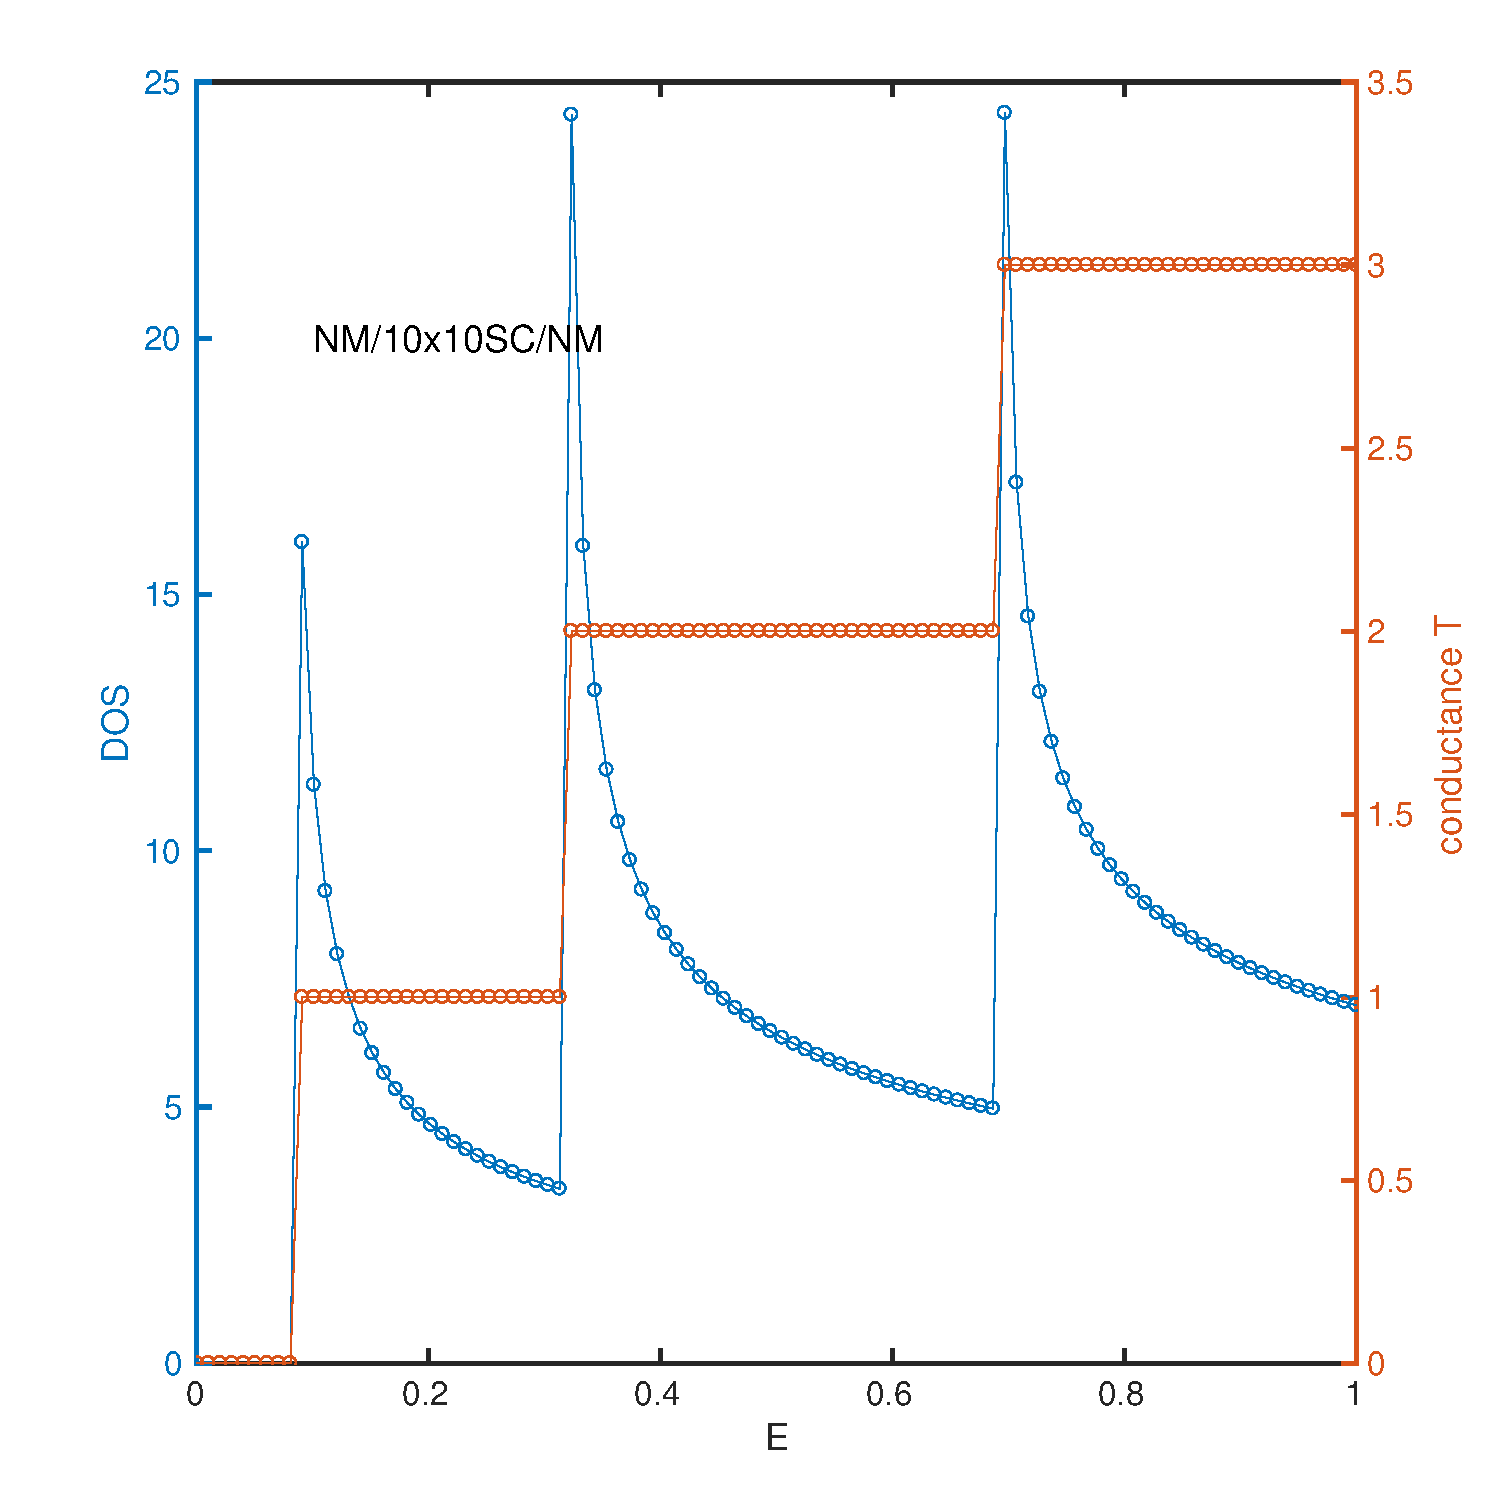
\includegraphics[width=0.5\textwidth, height=0.4\textwidth]{figures/DOST-E.pdf}
\caption{NM/10x10/NM system, 2D simple cubic lattice connected to two normal metal leads.}
\end{figure}
\subsection{NM/10x10SC/MI}
\begin{figure}[htp!]
\centering
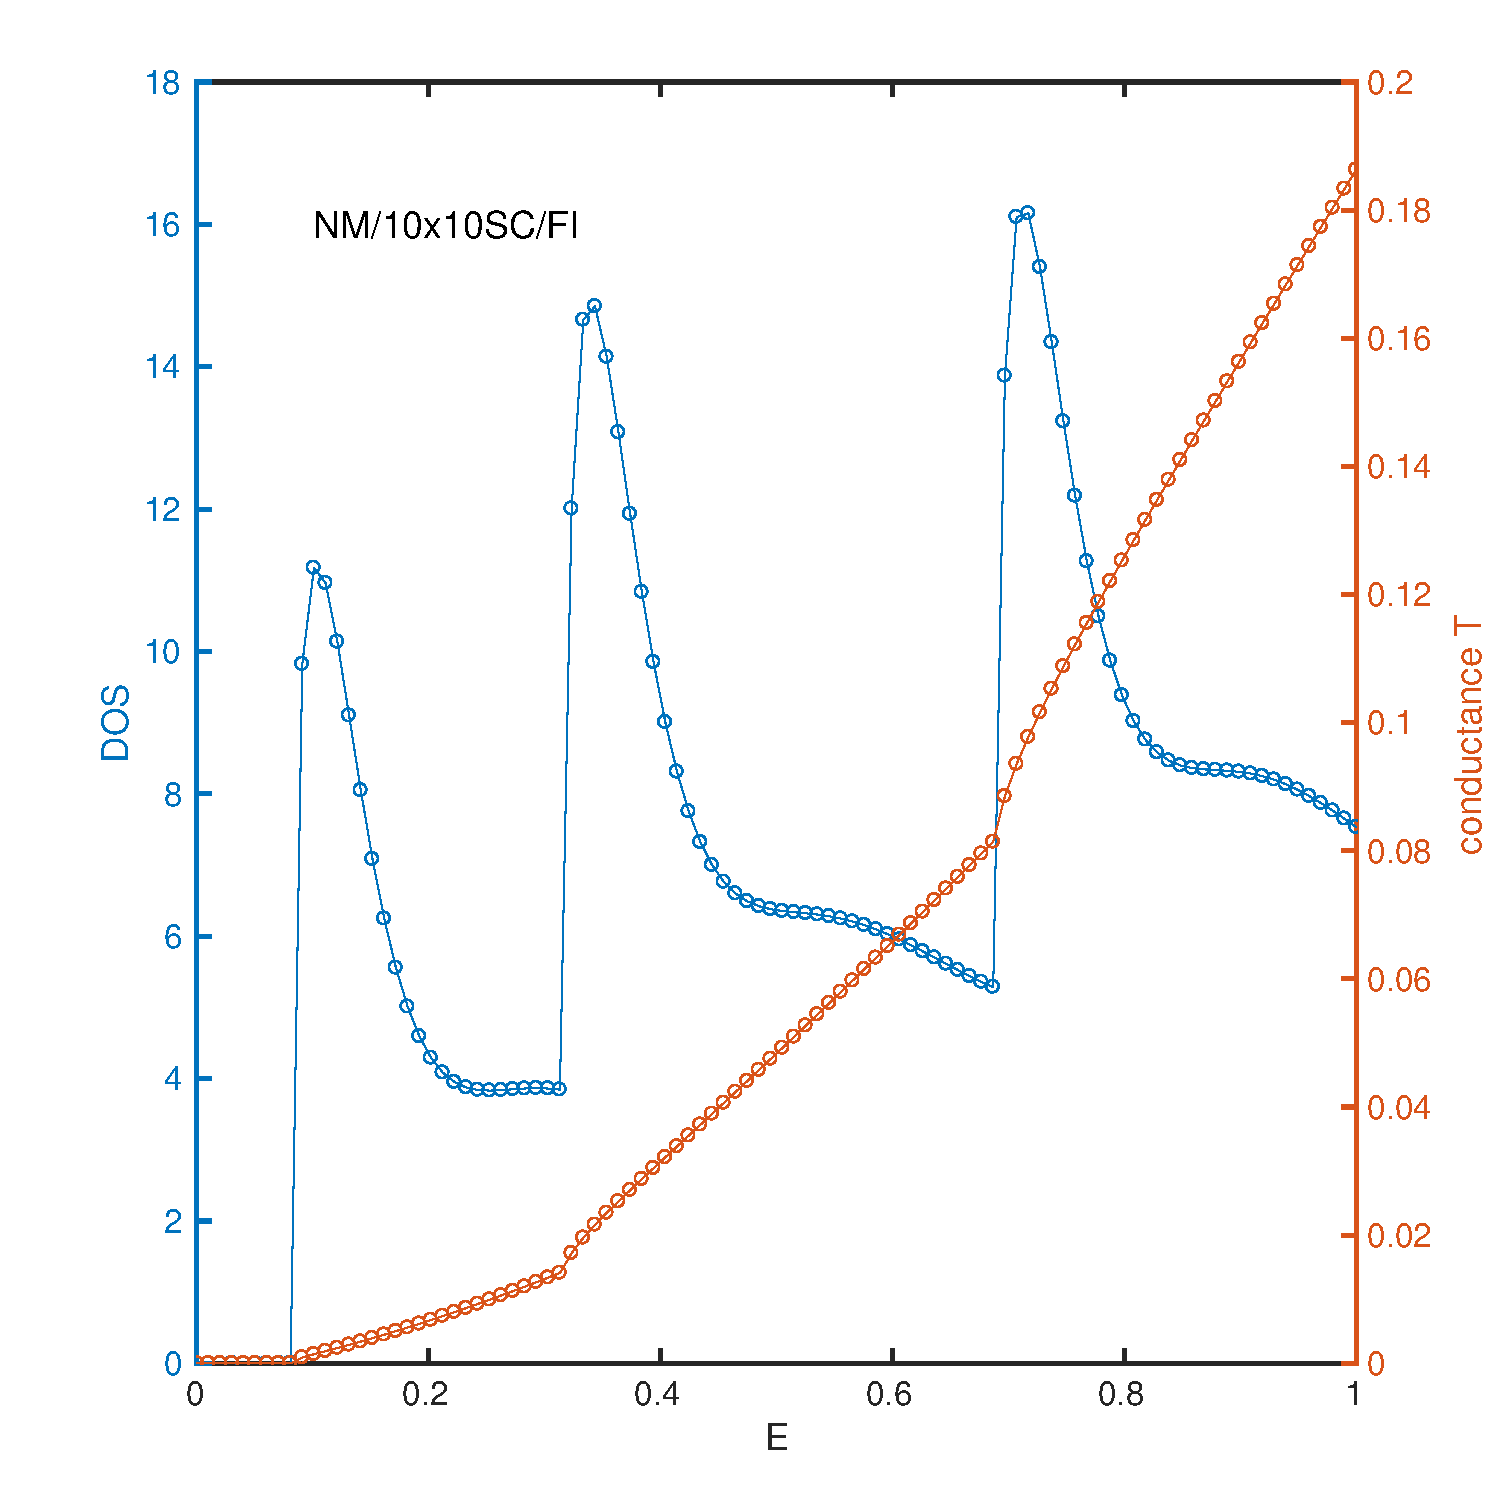
\includegraphics[width=\0.5\textwidth, height=0.4\textwidth]{figures/DOST-NM-FI.pdf}
\caption{NM/10x10/MI system, 2D simple cubic lattice connected to a normal metal lead and a magnetic insulator lead with Ohmic spectra.}
\end{figure}

\begin{thebibliography}{10}
\bibitem{ref1}
Y, K, Kato. Observation of the Spin Hall Effect in Semiconductors[J]. Science, 2004.
\bibitem{Jauho}
Antti-Pekka Jauho, Quantum Kinetics in Transport and Optics of Semiconductors, P188.
\end{thebibliography}

\end{CJK}
\end{document}


